%----------------------------------------------------------------------------------------
%	PACKAGES AND OTHER DOCUMENT CONFIGURATIONS
%----------------------------------------------------------------------------------------

\documentclass{article}
\usepackage{array}
\usepackage[english]{babel}
\usepackage[letterpaper,top=2cm,bottom=2cm,left=3cm,right=3cm,marginparwidth=1.75cm]{geometry}
\usepackage{amsmath}
\usepackage{graphicx}
\usepackage{float}
\usepackage[colorlinks=true, allcolors=blue]{hyperref}
\usepackage{todonotes}
\usepackage{setspace}
\onehalfspacing
\graphicspath{ {resources/} }

\title{Heimdall - A Kubernetes Extension}
\author{Bryan Keane}

\begin{document}

\begin{titlepage}

    \newcommand{\HRule}{\rule{\linewidth}{0.5mm}} 
    \center
    
    
    %----------------------------------------------------------------------------------------
    %	LOGO SECTION
    %----------------------------------------------------------------------------------------
    \begin{center}
        
\includegraphics{setu_logo.png}
    \end{center}
     
    %----------------------------------------------------------------------------------------
    
     
    %----------------------------------------------------------------------------------------
    %	HEADING SECTIONS
    %----------------------------------------------------------------------------------------
    \textsc{\Large Bachelor of Science (Hons) Applied Computing}\\[0.25cm]
    
    
    %----------------------------------------------------------------------------------------
    %	TITLE SECTION
    %----------------------------------------------------------------------------------------
    
    \HRule \\[0.75cm]
    { \huge \bfseries Heimdall - A Kubernetes Extension}\\[0.3cm] %document
    \HRule \\[1.0cm]
     
    %----------------------------------------------------------------------------------------
    %	AUTHOR SECTION
    %----------------------------------------------------------------------------------------
    
    \begin{minipage}{0.4\textwidth}
    \begin{flushleft} \large
    \emph{Author:}\\
    Bryan Keane 
    \end{flushleft}
    \end{minipage}
    ~
    \begin{minipage}{0.4\textwidth}
    \begin{flushright} \large
    \emph{Supervisor:} \\
    Lucy White
    \end{flushright}
    \end{minipage}\\[2cm]
    
\end{titlepage}

\newpage

\tableofcontents
\newpage

\listoffigures
\newpage




\section{Plagiarism Declaration}
I affirm that the work I am submitting is entirely my own and has not been taken from any other source, except where properly cited. I understand that plagiarism, collusion, and copying are serious offenses that can result in academic penalties. I have read and understood the assignment regulations and have properly cited all sources of information in my work. This assignment has not been previously submitted by me or anyone else for assessment on this or any other course.

\newpage
\section{Acknowledgements}
I would like to express my sincerest gratitude to my mentors, Ciaran Roche and Laura Fitzgerald, for their invaluable guidance and support throughout this project. Their expertise and knowledge have been integral to the success of this project, and I am deeply grateful for the opportunity to work with them. I would also like to extend my heartfelt thanks to my project supervisor, Lucy White, for her unwavering support and encouragement during this semester. Her guidance and assistance have been invaluable, and I am deeply appreciative of all that she has done to help me along the way. 


\newpage
\section{Introduction}
This project, Heimdall, is an open-source Kubernetes Extension built for multi-operator Kubernetes environments. Implementing Heimdall will allow developers to configure it to watch resources of their choosing in a Kubernetes cluster. Heimdall will prevent any unwanted Operators from changing that resource, while simultaneously sending an interactive notification to the developer via a pre-configured Slack Channel regarding the issue. 



\subsection{Background}
In 2022 I completed an 8-month internship at Red Hat for my 3rd-year work placement. I worked on the Red Hat OpenShift API Management (RHOAM) team. RHOAM utilises multiple OpenShift Operators, which are automatically managed and configured applications, to provide a comprehensive API solution to its customers. The API management features provided by RHOAM include: \cite{rhoam-overview}
\begin{itemize}
    \itemsep0em 
    \item Limiting the number of API requests based on the customer’s quota
    \item Creating security policies to manage API access
    \item Monitoring API health
    \item An API portal for sign-up and documentation
\end{itemize}
While working on this team, I had the opportunity to contribute to applications which utilize various technologies like Kubernetes, OpenShift, and Go Operators.



\subsection{Motivation} 
Throughout my internship, I ran into a number of technical issues. One such issue centred around RHOAM's rate-limiting service which has become the motivation for my final year project, Heimdall. The issue in question was with the port through which API requests were being sent in order to be rate limited. That port was being overwritten by a conflicting Operator who had a different desired state for that resource. Rate limiting in this context refers to the maximum number of API calls allowed during a specified time period \cite{understanding-apis} \\\par RHOAM uses the Marin3r Operator to provide rate-limiting for RHOAM customers. It works by injecting a rate-limiting container into a Pod. The container then acts as a middleman for API requests by only redirecting requests to the destination container if the API request limit has not been reached. A more detailed explanation of this process will be discussed in \hyperlink{technologies}{Section \ref{technologies}}. \\\par It took several days of debugging to figure out what was going wrong and another week passed before my fix was merged. This meant that this problem had been occurring on customer clusters before my fix was rolled out to production. After speaking to developers on various Red Hat teams, it became apparent that this problem was not unique to our team and in fact, was an issue that all Kubernetes and OpenShift product teams face. Fixing this will not only benefit Red Hat teams but any team working on a Kubernetes-based application that utilizes Operators.


\newpage
\subsection{Problem Statement} \label{problem-statement}
In Kubernetes (K8s), resources (or objects) have a desired state which describes what the actual state of that resource should look like. The desired state can either lie in a YAML definition or in the code of a Controller. Operators and Controllers can watch that resource's actual state and continuously compare it with the desired state. If they do not match then it is the job of that Operator or Controller to make the necessary changes in order to synchronise them \cite{operator-pattern}.

\begin{figure}[H]
    \hypertarget{problem-model}
    \centering
    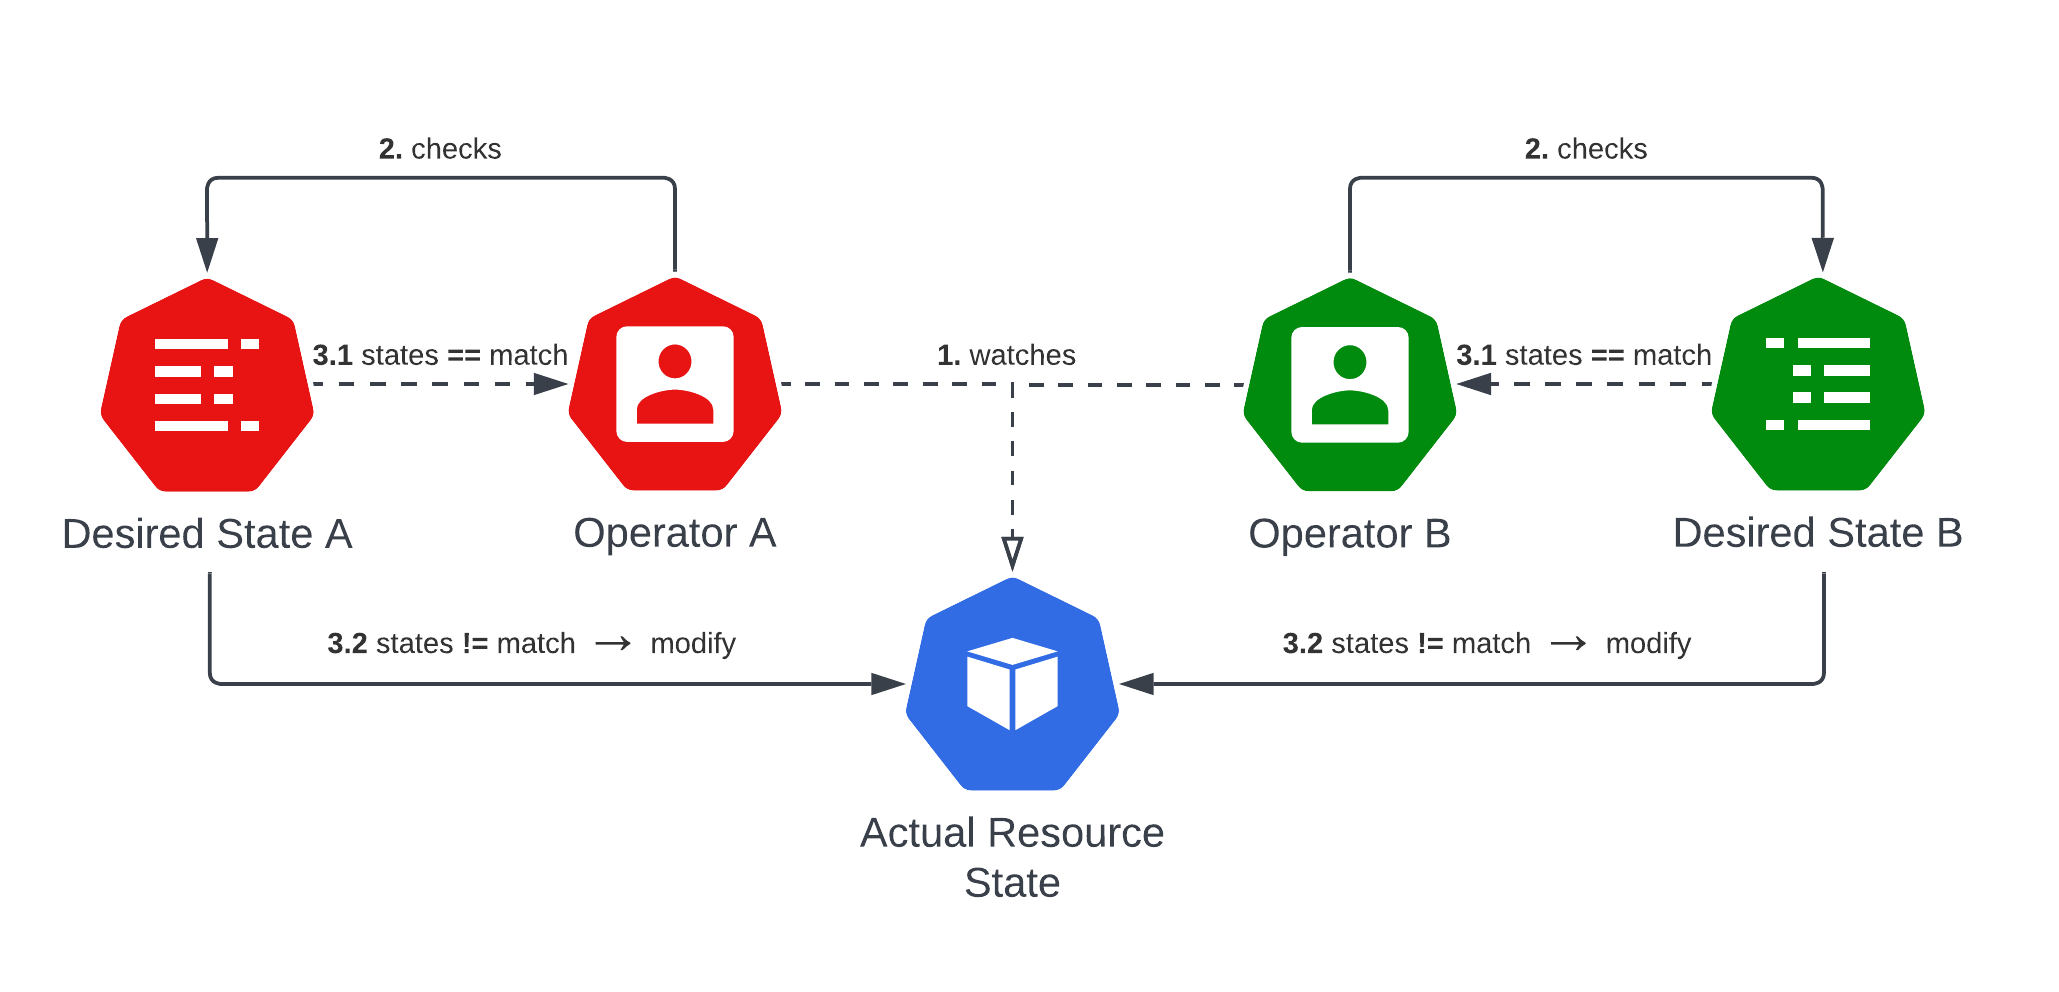
\includegraphics[width=150mm]{intro/problem-model.png}
    \caption{\emph{Model of The Problem - Two Operators Fighting Over a Resource's State}}
    \label{problem-model}
\end{figure}

This pattern works well until two Operators with conflicting desired states are both set to reconcile a resource. This will cause the resource's state to continuously change as both Operators attempt to synchronise its actual state with their unique desired state. The model shown in \hyperlink{problem-model}{Figure \ref{problem-model}} shows this problem in action. Each Operator will do the following:
\begin{enumerate}
    \itemsep0em 
    \item Watch a resource's actual state.
    \item Check the desired state for that resource.
    \item Compare the actual state with the desired state and
    \subitem 3.1. \emph{If they match} then return to Step 1. and repeat.
    \subitem 3.2. \emph{If they don't match} then modify the resource's actual state.
    \item Repeat this process continuously.
\end{enumerate}



\subsubsection{Industry Example}
As an example, the open-source e-learning platform Moodle can be used. In an educational environment, one might have a Moodle Operator and a MySQL Operator to serve as Moodle's database. The MySQL Operator manages the storing, of course, student, and module information. This application may then install a Tutors Operator, which is another e-learning platform which houses course notes and lab work. Since there is already a MySQL database via the MySQL Operator, Tutors can use the same database to store course notes and lab work. 

\begin{figure}[H]
    \hypertarget{moodle-tutors}
    \centering
    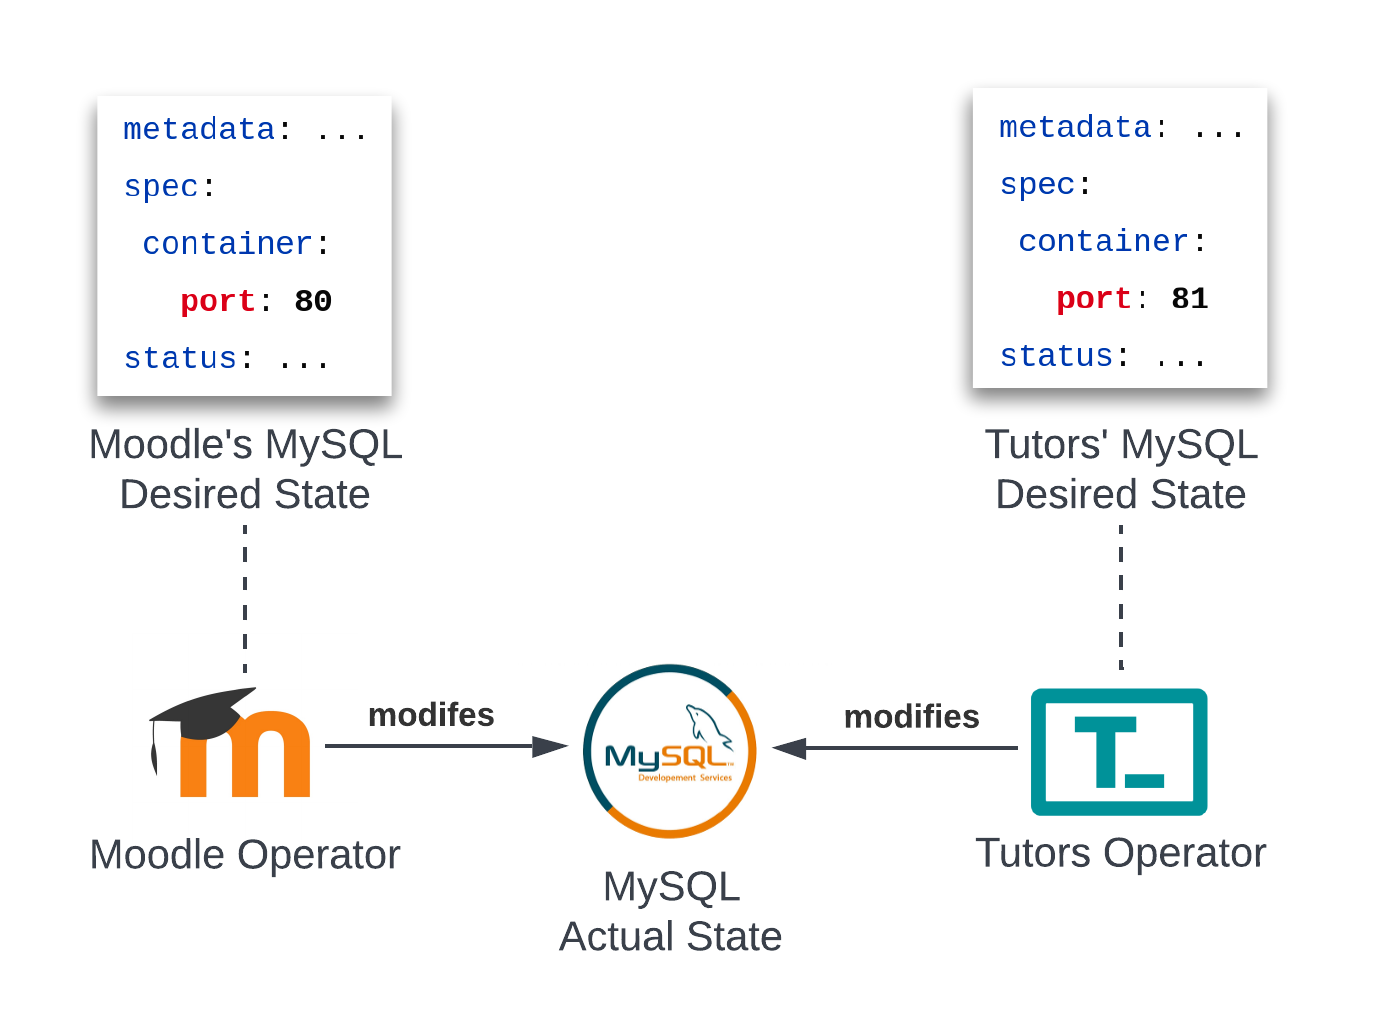
\includegraphics[width=125mm]{new-moodle-example.png}
    \caption{\emph{Simplified Model of Moodle, Tutors, and MySQL Industry Example}}
    \label{moodle-tutors}
\end{figure}

In this example, it would be very easy to misconfigure one of the Operators to have a dissimilar desired state for the MySQL resource. This would cause both Operators to constantly change that resource. Imagine Moodle wanted the port in which database access occurred to be port 80 and Tutors wanted the database access to occur through port 81. This would cause the MySQL resource's access port to be changed back and forth. If a lecturer or student attempts to access information through Moodle, but at that point in time the MySQL resource's port was configured by the Tutors Operator, the user would not be able to retrieve the data. 

\subsection{Aims and Objectives} \label{aims-and-obj}
The solution is to create a custom Kubernetes controller which will monitor resource states. A Kubernetes Operator can create a resource, become its owner, and will set the controller to watch that resource for changes. If another operator changes the resource the controller will trigger an alert, notify the developer via a slack integration and allow the developer to fix the problem without the need for time-consuming debugging. 

\begin{figure}[H]
    \hypertarget{solution-model}
    \centering
    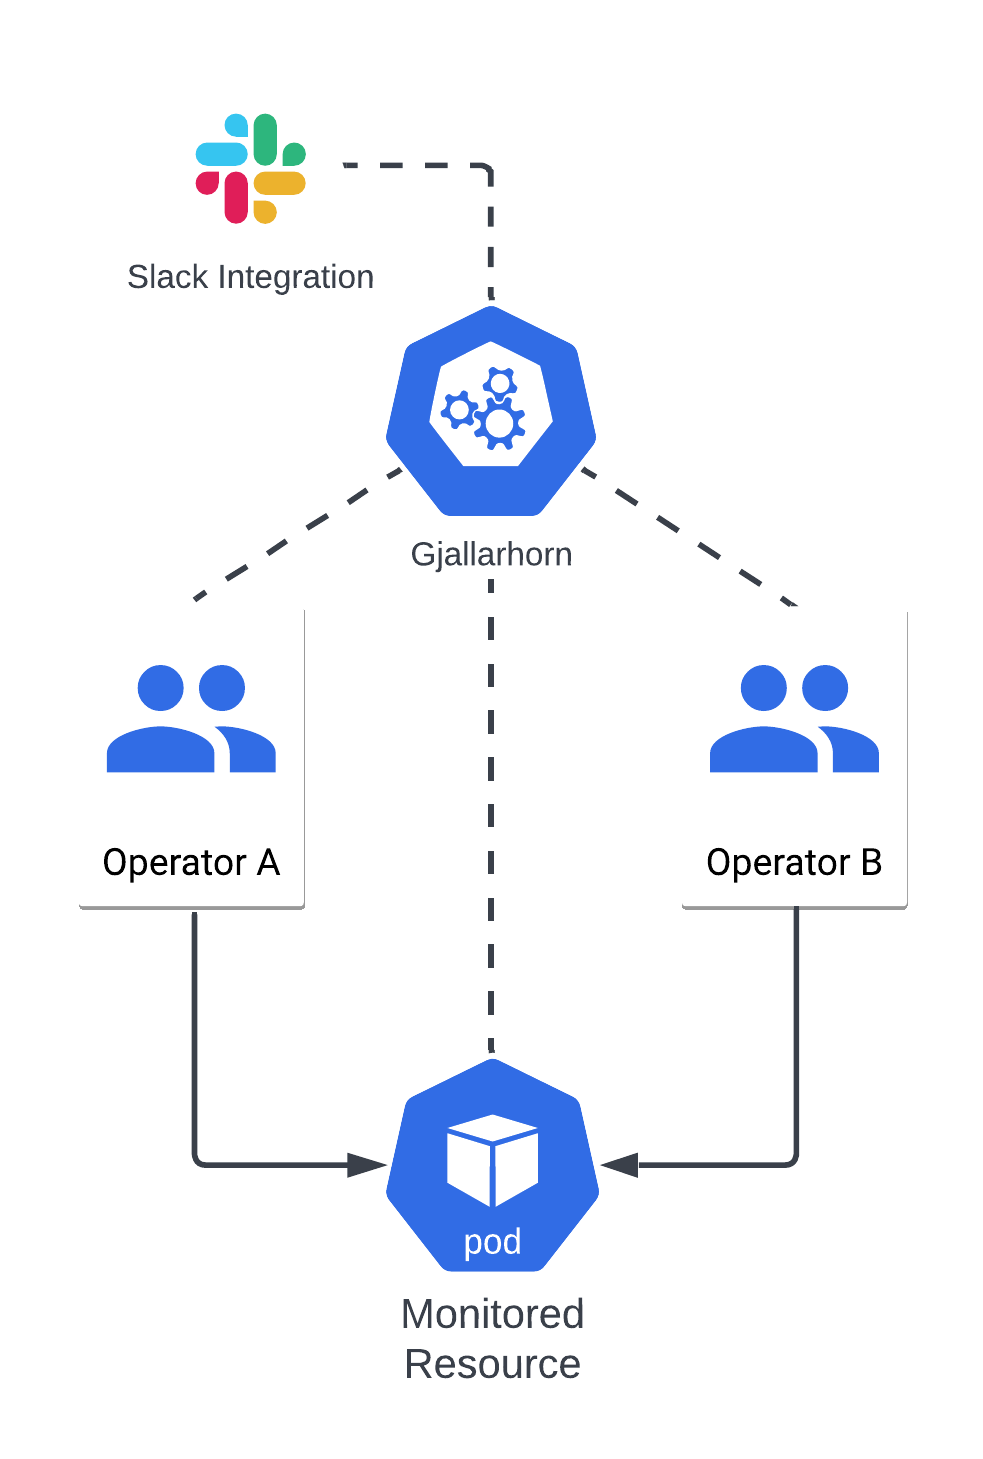
\includegraphics[width=100mm]{solution-model.png}
    \caption{\emph{Model of the solution: Heimdall}}
    \label{solution-model}
\end{figure}

\hyperlink{solution-model}{Figure \ref{solution-model}} models the proposed solution where the Owner Operator and Rogue Operator are attempting to change a resource's actual state. Once the Owner Operator is installed, it creates the resource with the addition of a label that Heimdall is looking for. Heimdall sees a new resource created with this label and begins monitoring its state. The Rogue Operator is installed and begins changing the resource. \\\par The minimum viable product for Heimdall involves the controller watching for non-owners changing the state of a resource. It will then generate an interactive notification for slack with details on the issue to allow the developers to find and fix the problem with relative ease. The stretch goals for Heimdall will achieve the following:
\begin{enumerate}
    \itemsep0em 
    \item Allow for an atomic owner of a resource to be set.
    \item Block changes to resources from non-owners.
\end{enumerate}

This will not only allow the developer to fix the problem with ease but also stop the issue from occurring and prevent any downtime for the end user.


\newpage

\section{Design}

This section will provide an overview of the Heimdall controller, including its architecture and technical components. It will also delve into the details of each aspect of the project to give a full understanding of its function and purpose.


\subsection{Requirements} \label{requirements}

There are various requirements for the successful implementation of Heimdall. These requirements can be divided into two categories: functional requirements and non-functional requirements. Functional requirements describe the specific capabilities or features that the system must have, while non-functional requirements describe constraints that the system must adhere to \cite{func-vs-nonfunc}. It is important to carefully define both types in order to ensure that Heimdall meets the needs of its users and operates in a reliable manner. These will serve as a guide for the development of the Controller and will help to ensure that it is able to effectively detect and resolve conflicting Resource changes between Operators in a Kubernetes cluster.


\subsubsection{Functional Requirements}

Functional requirements are features and capabilities that the system must possess in order to meet the needs and expectations of the user. In the case of Heimdall, these requirements are primarily focused on the functionality that will be most useful to developers implementing the controller into their environments, as well as site reliability engineers installing it onto customer Kubernetes clusters. Heimdall's Functional Requirements are as follows:

\begin{enumerate}
    \itemsep0em
    \item Developers must be able to install the controller on any Kubernetes cluster.
    \item Developers must be able to configure the controller to connect to Slack for notifications.
    \item Developers must be able to define an Operator that is unable to make changes to the specified Resource.
    \item Developers must have access to appropriate documentation which outlines the proper configuration and use of Heimdall.
\end{enumerate}

With the functional requirements outlined, the following section will delve into the technical details necessary for the successful implementation of these end-user features.

\subsubsection{Non-Functional Requirements}

Non-Functional Requirements are technical specifications that help ensure that the system meets the desired functional requirements. They define the performance, reliability, security, and other characteristics that the system must possess in order to function effectively. Heimdall's Non-Functional Requirements are as follows:
\begin{enumerate}
    \itemsep0em
    \item Heimdall must be able to use the Unstructured Package to watch Resources of any type, including Core and Custom Resources.
    \item When a Resource is watched, events on it should trigger a Reconcile for that Resource.
    \item During a Reconcile, Heimdall must verify if events are coming from the owner Operator or not.
    \item If the event is coming from a non-owner, Heimdall must configure a new Role and Role Binding to grant the correct permissions to that Operator's Service Account.
    \item The Controller must also handle the reconciliation of the Slack integration, including:
    \subitem a. A Config Map storing the Slack channel information that Heimdall sends notifications to.
    \subitem b. A Secret storing the Slack API Key that Heimdall uses to send Slack messages.
    \item Heimdall must use the Slack Go Client to send messages to a Slack Channel with information from the Config Map and Secret.
    \item These messages must be interactive and provide a link to the affected Resource.
    \item Finally, Heimdall must have a working and publicly available Docker image built for installation.
\end{enumerate}

These requirements provide the foundation for the design of the system, as they outline the necessary capabilities and technical considerations that must be taken into account. In the following section, we will delve deeper into the architecture of Heimdall and discuss how these requirements will be implemented and integrated into the overall design of the system.

\subsection{Architecture Model}

The design of Heimdall is shown in Figure \ref{arch-diag}, which illustrates the controller's functions and responsibilities in an example scenario. In the following section, we will explore the components and processes of Heimdall in more detail to understand how the controller functions and meets its requirements.

\begin{figure}[H]
    \centering
    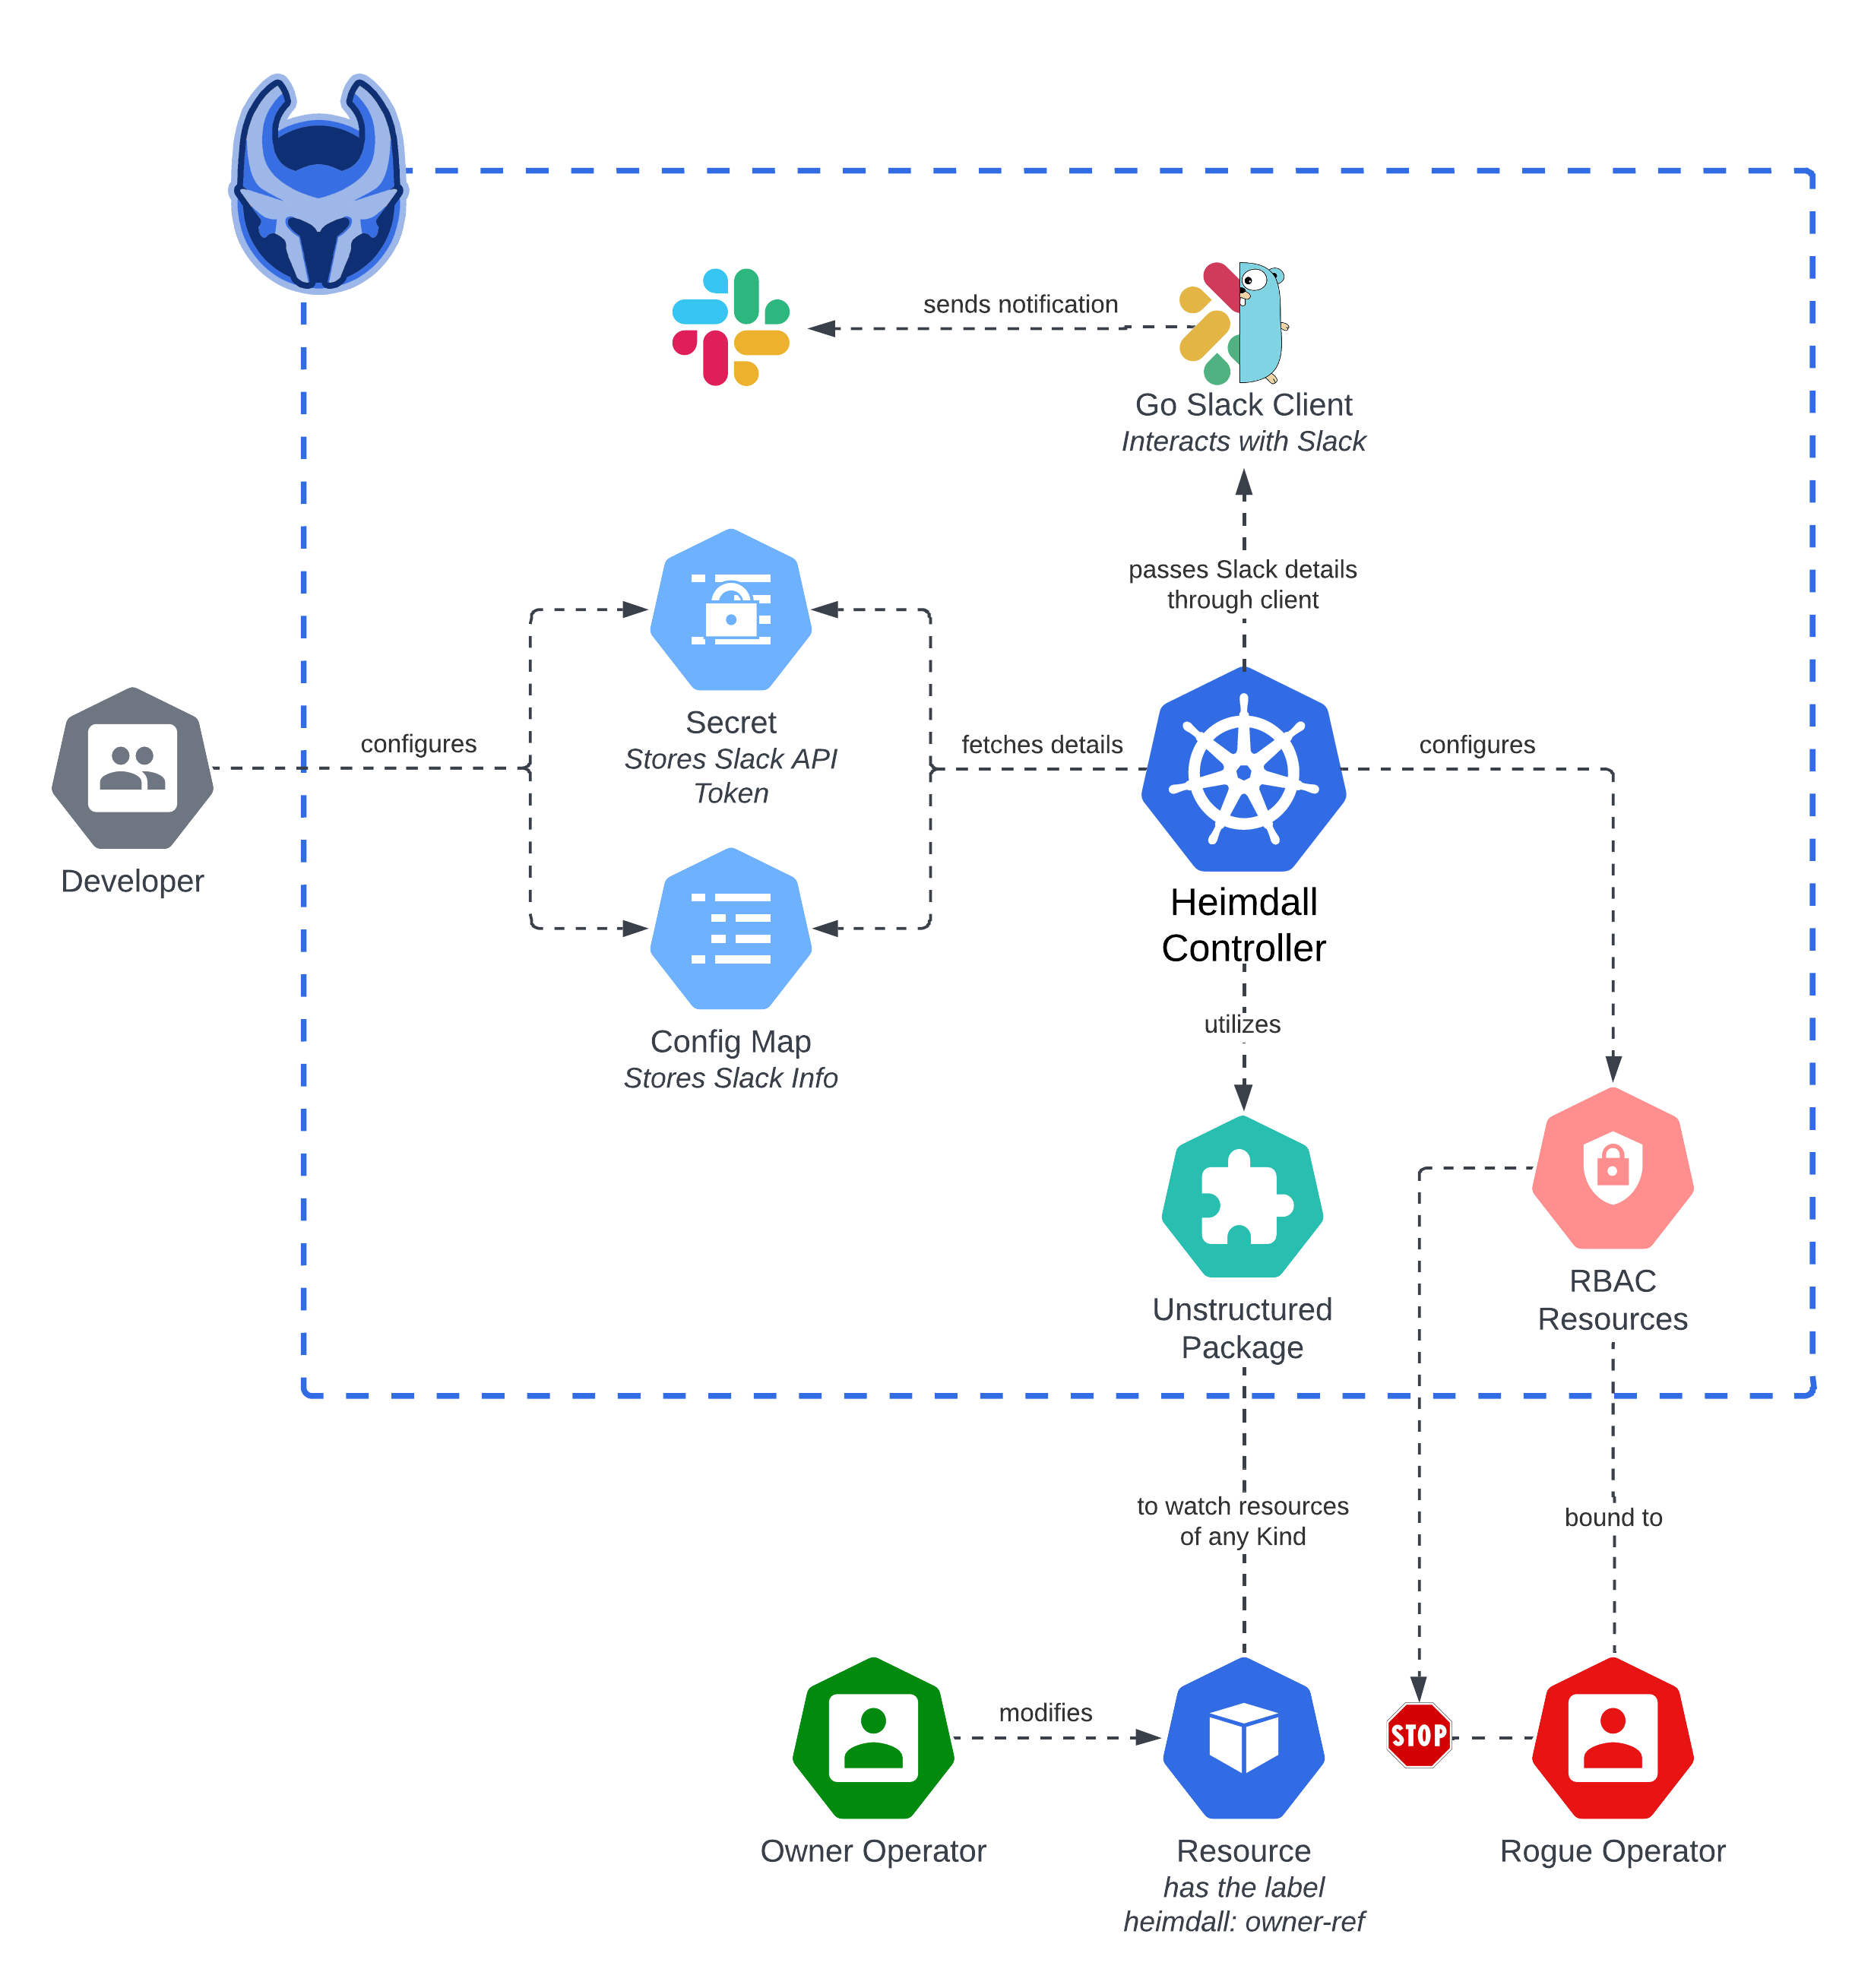
\includegraphics[width=160mm]{design/arch-diag.png}
    \caption{\emph{Heimdall system architecture overview model}}
    \label{arch-diag}
\end{figure}


\subsection{System Design} \label{design-desc}

The system design aims to provide a detailed description of the various components involved in the implementation of Heimdall. This section will cover the Controller Overview, the use of the Unstructured Package, Slack Integration, Role Based Access Control, and Installation. 

\subsubsection{Controller Overview}

The Controller is the main component of Heimdall. It initializes using the \emph{controller-runtime} package, which is discussed in Section \ref{osdk}, and sets a Watch on specific Resources using the Unstructured Package. When an event occurs on a Watched Resource, the Reconcile function carries out the logic to identify whether the change came from the owner or a rogue Operator. If it is a rogue Operator, it will trigger a Slack Notification and reconfigure Role-Based Access Control Resources to block any future changes from that Operator.

\subsubsection{Unstructured Package Implementation}

As part of the Heimdall Controller, the Unstructured package must be used in order to Watch Resources of any type in a Kubernetes cluster. This package provides a means by which to convert any type of Object in a Kubernetes cluster and turn it into a generic type. This will allow Heimdall to not have to declare the resource type when setting a Watch on Resources, so it can essentially Watch any resource in a cluster. This is especially helpful for Custom Resources as Heimdall needs to be installed and configured to work with any Kubernetes environment, so it needs to be dynamic in the way that it deals with Resources of different types.

\subsubsection{Slack Integration}

The integration with Slack involves a few different steps. The main components are the Config Map, the Secret, and the Slack Go client. Heimdall will first need to Reconcile the Config Map and the Secret. If either of them does not already exist in the cluster, the Controller will create them. This is so both Resources are guaranteed to be present on the cluster and ready for the Developer to configure them. Once they are configured correctly with the Slack API Token and the Slack Channel name, Heimdall can use that information to send Slack messages. The messages sent will need to be somewhat interactive. Ideally, this would include a link to the affected Resource, but at the very least it should contain the Name and Namespace of the Resource, the event type, and the source of the unwanted changes.

\subsubsection{Role Based Access Control} \label{security}

Upon a watched Resource being changed by a non-owner, Heimdall will detect that change and trigger the Reconcile function for that Resource. To stop any new changes from being made by that Operator, the Controller must create new RBAC Resources like Roles and Role Bindings. The Roles will be bound to the Operator's Service Account with new Role Bindings so that when that Operator attempts to make another change to the watched Resource, it won't have the correct permissions. This functionality is subject to change as it has not yet been attempted and is not confirmed to be possible in a production environment. Upon actually implementing this functionality, it may differ slightly from this design.


\subsubsection{Installation}

Lastly, Heimdall needs to be installable via a public Docker image. An image can be built and pushed to a public container image repository like Docker Hub or Quay. This image can then be used by any developer that needs to implement Heimdall into their environment and run on the cluster. Appropriate documentation will need to exist so that the installation and configuration are easy to complete. This documentation should also include steps to create a Slack API for the developer's Slack Channel, and how to configure the Config Map and Secret correctly.



\subsection{User Stories}

User stories are a way of expressing requirements for a product in a way that is easily understood by a product's stakeholders. They are used in Agile development, as discussed in Section \ref{agile}, and are an important tool for creating a shared understanding of the desired functionality of a product \cite{user-stories}. User stories help to focus on the value that a feature will provide to the end user and provide a framework for refining its requirements. The following are Heimdall's user stories:

\begin{itemize}
    \itemsep0em
    \item As a Developer, I want to be aware of changes to resources that I own so that I can take action if an unwanted change is made.
    \item As a Developer, I want to control the cadence of alerts so that I can control the noise created by those alerts.
    \item As a Developer, I want to claim ownership of the resources that I control.
    \item As a Developer, I want to control the changes to resources that I own.
\end{itemize}

These provide clear and concise descriptions of the desired functionality of Heimdall and will serve as a guide for the development team next semester.

\subsection{Risk Analysis}

There are a number of risks associated with this project's implementation, one of which is far more significant than the others. During initial research, there were no examples or previous attempts found to implement such a solution, posing a significant risk that it may not be technically possible. To mitigate this, the project has been split into a Minimum Viable Product (MVP) and stretch goals. If the MVP can still be completed, it will still provide a valid solution. If the implementation is confirmed to be possible, the next risk is that the project cannot be completed within the given time constraint. However, with the use of the methodologies discussed in Section \ref{methodology}, the use of Sprints, and using CI/CD for development should mitigate any concerns about time. After completing the RBAC Prototype seen in Section \ref{rbac-prototype}, it is likely that the Stretch Goals will be feasible in some form.


\section{Methodology} \label{methodology}

This section will outline the Agile methodology that has been adopted for the development of Heimdall, as well as the version control, continuous integration, and continuous delivery practices that will be implemented to ensure the smooth development of the project. Additionally, we will delve into the testing approach taken and the decision to open-source the project.


\subsection{Agile and Scrum} \label{agile}

Agile is a project management and development method that helps teams deliver value to customers more efficiently. It is based on the idea of continuously iterating on and improving a product through the collaboration of teams \cite{what-is-agile}. Agile has been chosen because it allows for a more flexible approach to development. By focusing on delivering the most important features first, there is a higher probability of being able to successfully implement the MVP and Stretch Goals. \\\par Scrum on the other hand is a framework for Agile development that emphasizes collaboration, flexibility, and the ability to respond to change. One way that Agile teams track progress is through the use of Scrum artifacts such as Burn-down charts and Velocity Reports. While the Scrum roles may not be applicable to a one-developer project like Heimdall, the use of these artifacts will still be useful in monitoring progress and ensuring that the project stays on track.


\subsection{Scrum Artifacts} \label{artifacts}

Scrum Artifacts are essential tools for Agile teams. They provide a way to track and communicate the progress of a product. During this project, several Scrum Artifacts including Backlog Refinement and Sprint Reviews were used. These artefacts helped to plan and execute work effectively. The use of these artefacts can aid in the improvement of a developer and should showcase the development of skills as time goes on.

\subsubsection{Sprints, Sprint Reviews, and Backlog Refinements}

The management of work for Heimdall was initially conducted through weekly Sprints. However, in order to more effectively track progress and allow for regular meetings with the Supervisor, the decision was made to switch to bi-weekly Sprints. This allowed the meeting at the end of each Sprint to serve as a Sprint Review, which is a regular meeting that allows teams to review progress and make adjustments \cite{scrum-guides}. The meeting during the Sprint served as Backlog Refinement, which is an ongoing activity in which teams discuss tickets in order to improve accuracy \cite{scrum-guides}. The bi-weekly Sprints allowed for constant progress tracking and the ability to make necessary adjustments as needed. A Sprint Review document was kept as a log of the weekly Sprints and Sprint Reviews, which can be seen in Appendix \hyperlink{appendix-f}{F}.


\subsubsection{Burn-down Charts} \label{bdc}
Burn-down charts are a chart of the remaining story points for a sprint. The goal for these charts is a steady downward trend throughout the sprint ending with little to no story points left. The burn-down chart for the first two Sprints (week one and two) can be seen in Figure \ref{s1ands2bd}.

\begin{figure}[H]
    \centering
    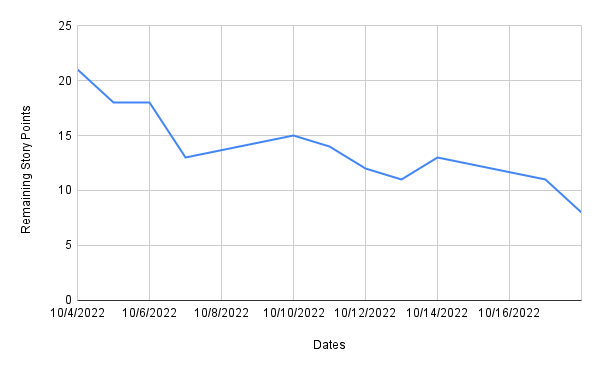
\includegraphics[width=120mm]{methodology/s1and2bd.png}
    \caption{\emph{Sprint 1 and 2 Burndown Chart}}
    \label{s1ands2bd}
\end{figure}


Comparing charts can be a useful way to track progress and improvement over time. For the first two Sprints, the estimation for the number of story points that could be completed was too high, and only about half of the estimated work was actually finished. In contrast, in the Burn-down chart for the most recent Sprint in Figure \ref{s7bd}, the estimation for the number of story points that could be completed was higher than in the first Sprints, and all of the estimated work was completed. This indicates an improvement in both estimation and rate of work completion. 

\begin{figure}[H]
    \centering
    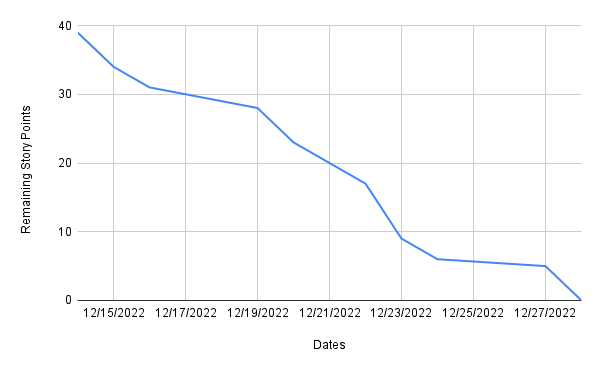
\includegraphics[width=120mm]{methodology/s7bd.png}
    \caption{\emph{Sprint 7 Burndown Chart}}
    \label{s7bd}
\end{figure}

While Sprint 7 is near the end of the Semester, so it should be assumed that all story points were completed, ideally next semester each sprint will reflect a more accurate estimation similar to Sprint 7's.

\subsubsection{Velocity Report}

Velocity Reports help predict future workload by tracking work completed in previous sprints. The report in Figure \ref{velocity} shows the number of story points completed in each sprint. By analyzing this data, adjustments can be made to improve estimation accuracy and increase productivity. This can be useful for planning future sprints, including those in the next semester.

\begin{figure}[H]
    \centering
    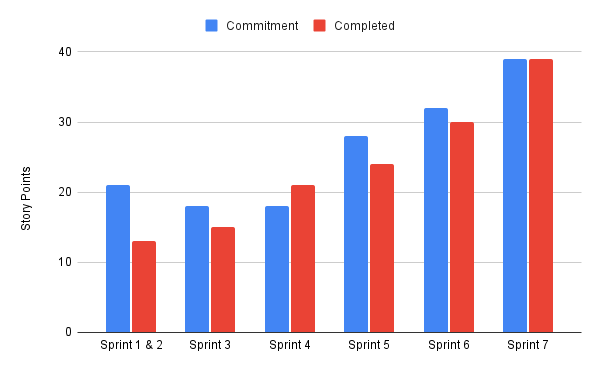
\includegraphics[width=120mm]{methodology/velocity.png}
    \caption{\emph{Sprint Velocity Report}}
    \label{velocity}
\end{figure}


\subsection{Version Control} \label{version-ctrl}
Version Control is a method in which changes to files are recorded over time so they can be reverted or referenced if needed. It is typically used in software development to track changes to source code. In this project, Git and GitHub are used for version control. Further details can be found in Section \ref{gha}. Heimdall's code is stored in a GitHub organization seen in Appendix \hyperlink{appendix-a}{A} to mimic how real products in companies are managed on GitHub. Every piece of work is merged as a pull request, which allows for review and checking before merging, allowing for easy reverting in case of any issues that may arise after a commit.

\begin{figure}[H]
    \centering
    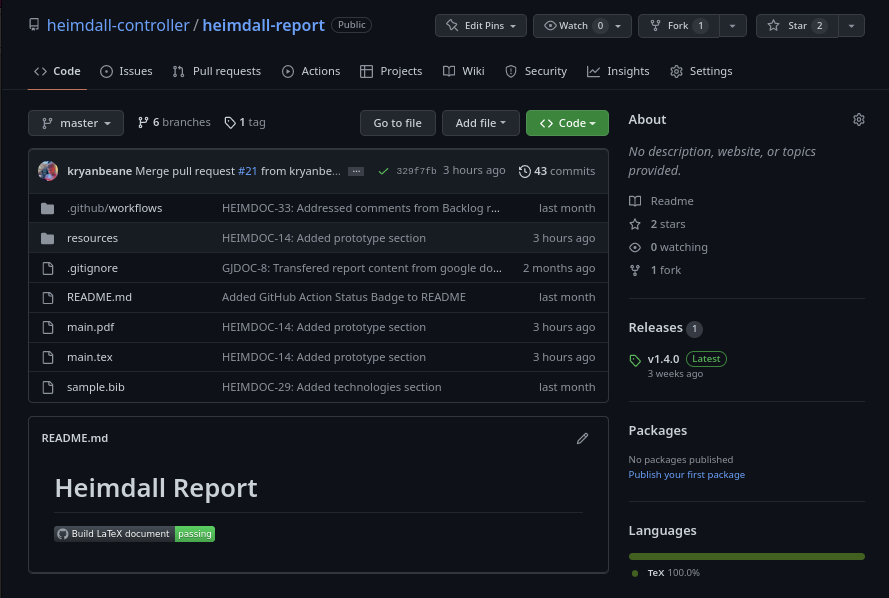
\includegraphics[width=120mm]{methodology/github.png}
    \caption{\emph{Heimdall Report GitHub Repository}}
    \label{github}
\end{figure}



\subsection{CI/CD} \label{cicd}

Continuous Integration and Continuous Delivery (CI/CD) are two key practices that are essential for the efficient development and delivery of a product. CI refers to the practice of regularly integrating code changes into a repository, while CD refers to the practice of automatically building, testing, and releasing code changes \cite{ci-cd}. Together, these practices help ensure that code can be quickly and easily tested, validated, and deployed to production environments. To streamline development and deploy updates to Heimdall efficiently, CI/CD practices are being implemented. This includes automating testing and building with GitHub Actions, with plans to also use it for releases. By automating these processes, delivering new functionality and completing the MVP and Stretch Goals should be unproblematic.


\section{Technologies} \label{technologies} 

The selection of technologies for a project plays a crucial role in determining its success. It is important to carefully consider the capabilities and limitations of various technologies, as well as how they will integrate with one another, in order to build a solution that meets the project's needs. The following is an extensive list of the technologies chosen to implement Heimdall, each one carefully selected to best fit the needs of the project.

\subsection{Kubernetes}

Kubernetes is an open-source tool used to implement modern micro-service-based architectures. It can be used to create, manage, and deploy containerized applications and is commonly known as a container orchestrator \cite{k8s-overview}. Containers are small processing units which house applications and their dependencies. They are bundled up into a singular image that is able to run on any hardware. This removes the need for installing required packages when attempting to run an application. Kubernetes orchestrates the deployment of many containers to form larger applications that are highly available, fault-tolerant, and have high degrees of redundancy.


\subsubsection{Resources} \label{resources}

Resources, also known as objects, are how the state of a Kubernetes cluster is represented. These resources are detailed in \emph{.yaml} format \cite{k8s-obj}. They usually describe the following key pieces of information:

\begin{itemize}
    \itemsep0em 
    \item Which container image is being used
    \item The compute resource available to the application, namely CPU and Memory limits
    \item Resource policies on how things like fault tolerance, upgrade behaviour, and restart behaviour should operate
    \item General resource information like the Namespace, Labels, and Annotations
\end{itemize}

The lowest-level Kubernetes resource is a Pod. Pods house the containers that run applications. They are expendable and can never be edited. If the desired state of a Pod is changed, it is destroyed and recreated to match the Pod's actual state with the new desired state. This also increases the cluster's degree of fault tolerance as if one Pod fails, instead of trying to recover it the Pod can be deleted and redeployed. 

\begin{figure}[H]
    \centering
    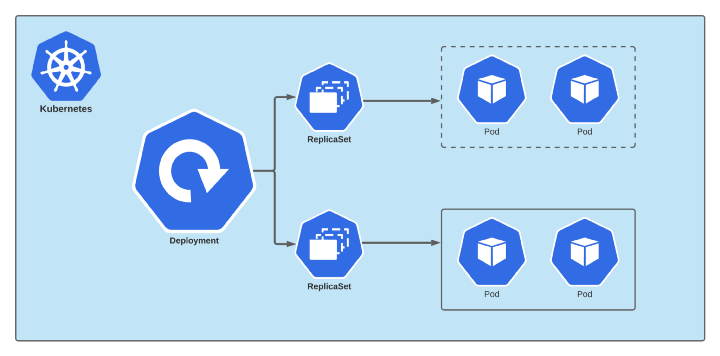
\includegraphics[width=160mm]{tech/resource-struct.png}
    \caption{\emph{Kubernetes application Resources: Deployments, Replica Sets, and Pods}}
    \label{resource-struct}
\end{figure}

There are two other Resources which make up the structure of a running application in Kubernetes. Figure \ref{resource-struct} \cite{k8s-rolling} details how Deployments and Replica Sets work with Pods in order to complete an application's workflow. Deployments are the top-level Resources in this structure and typically act as the source of truth (desired state) for Pods. If a Deployment's \emph{.yaml} specification is changed by another Controller, then its Pod's desired state will change and be redeployed. The Deployment also acts as a desired state for Replica Sets, which are responsible mainly for managing the number of Pod replicas currently running. 

\begin{figure}[H]
    \centering
    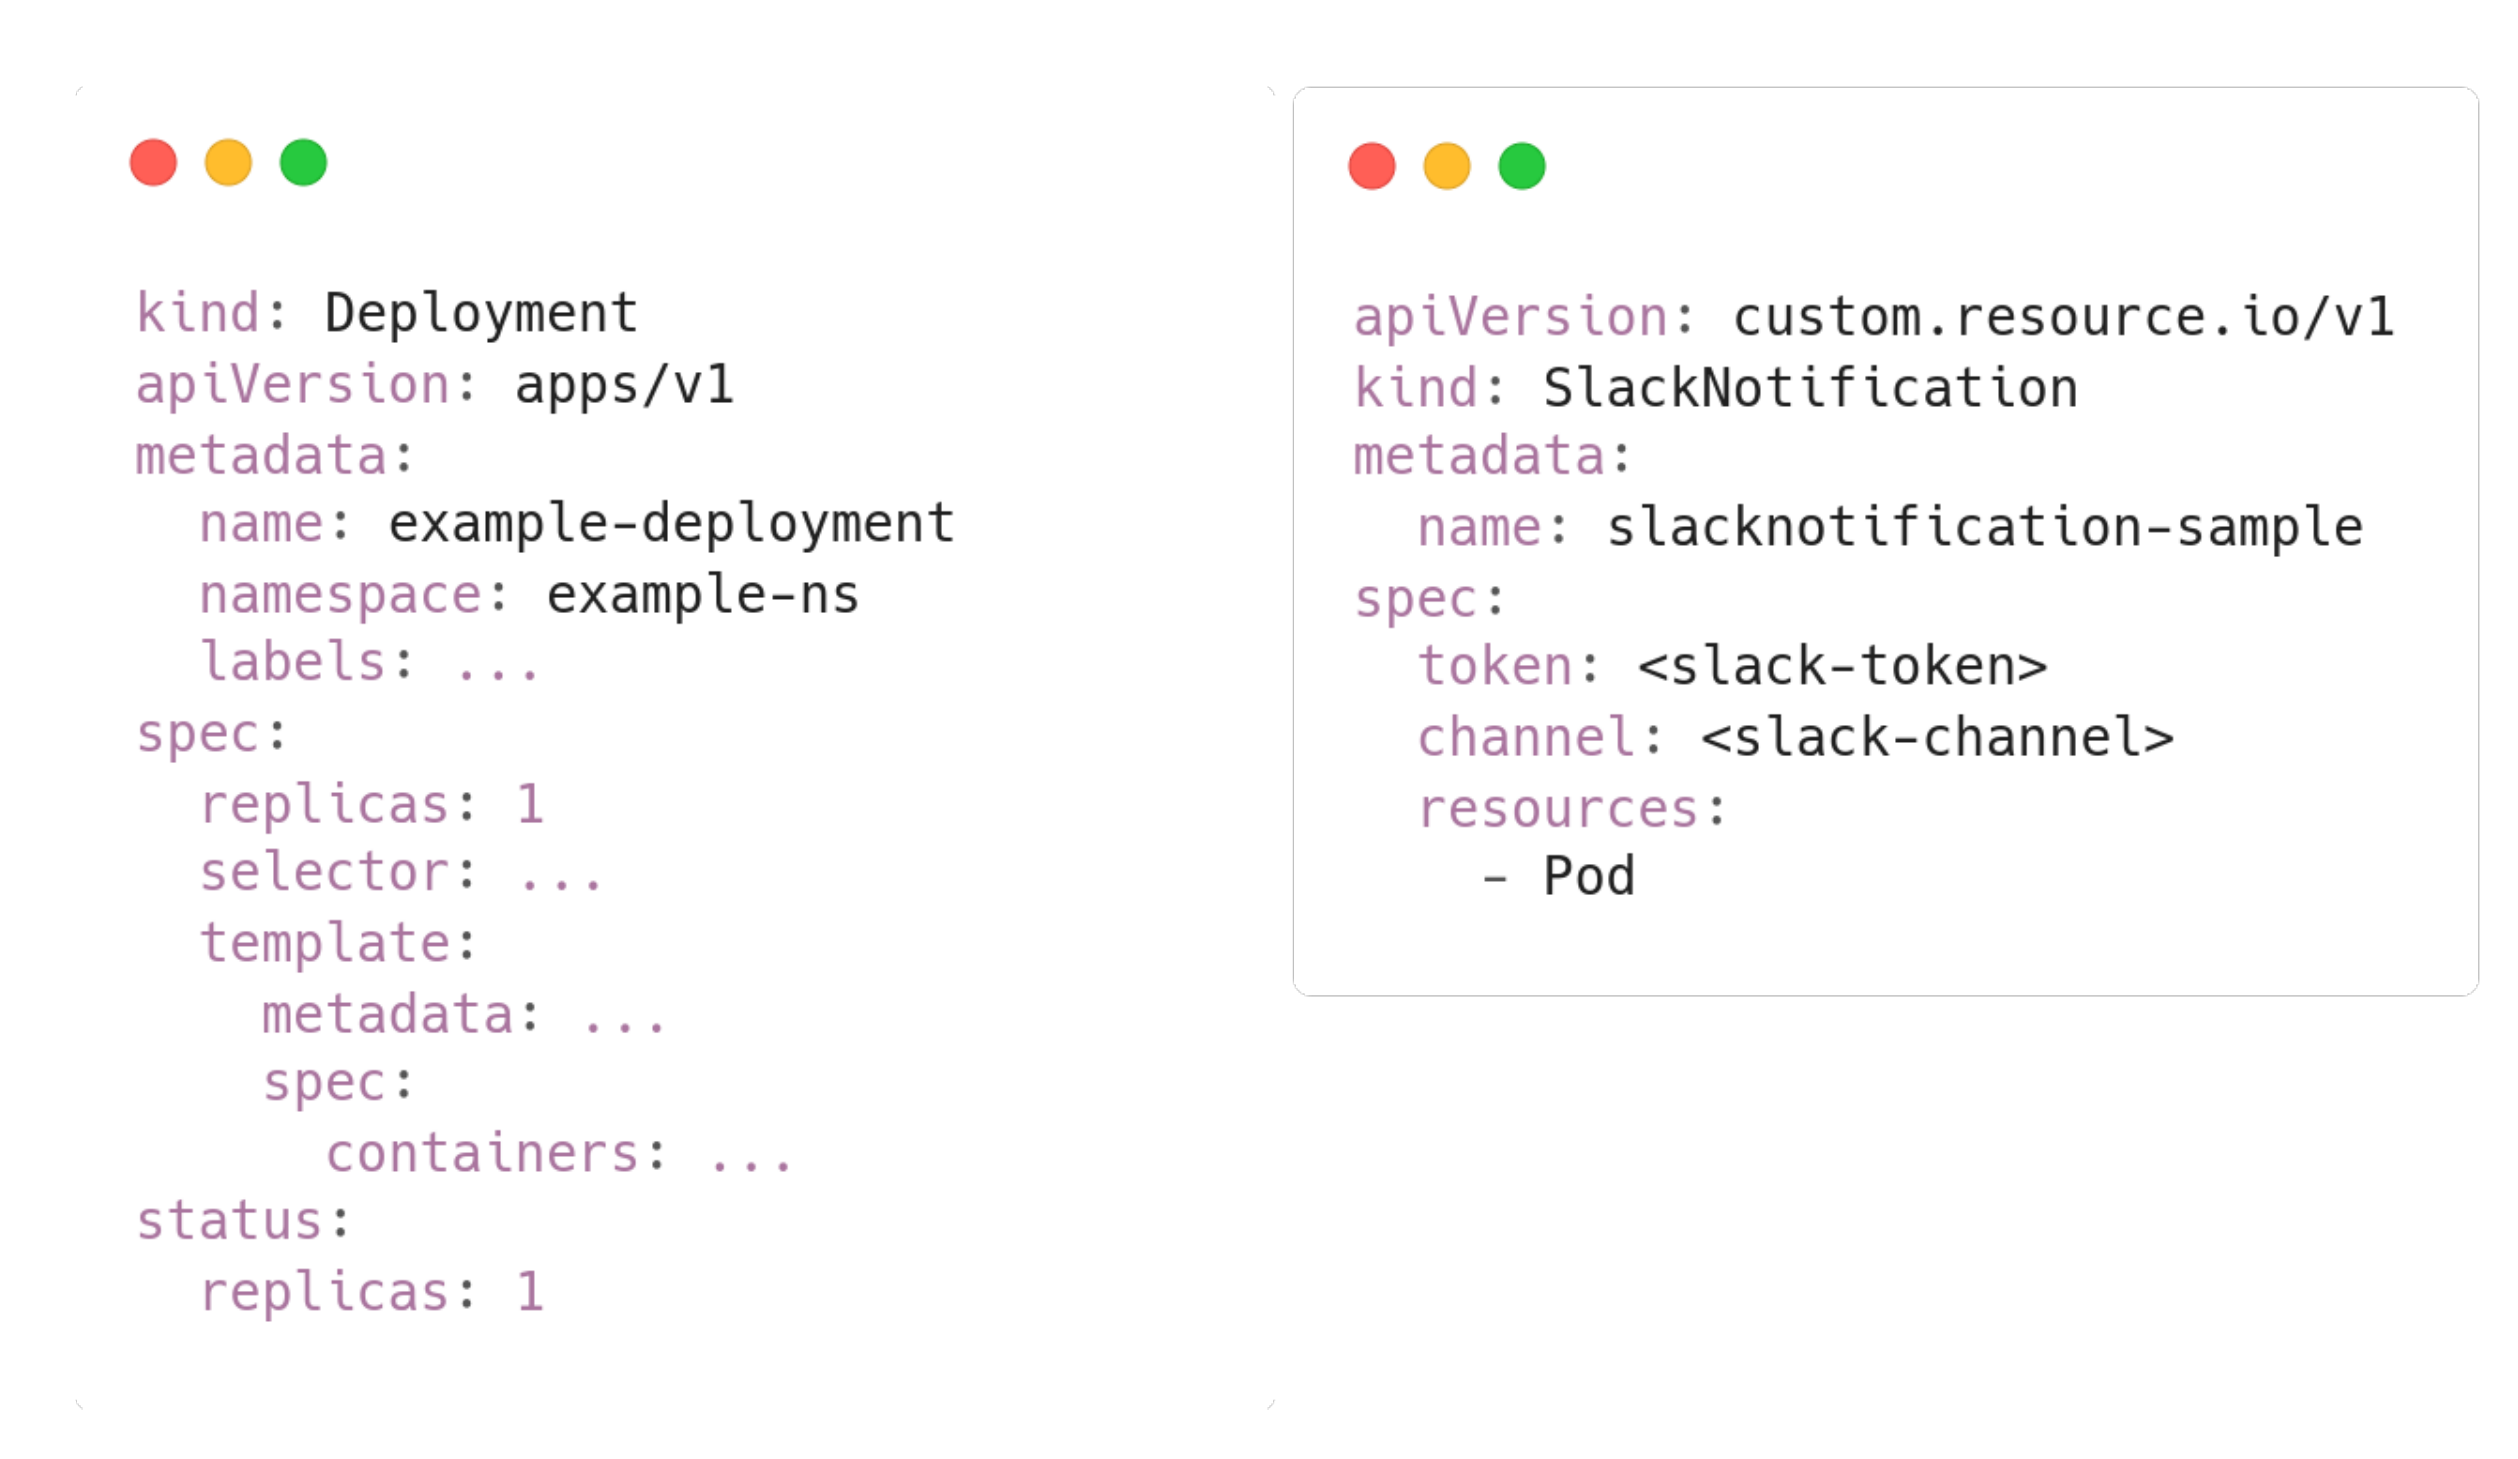
\includegraphics[width=125mm]{tech/core-cr.png}
    \caption{\emph{Example Core Resource (Deployment) comparison with Example Custom Resource}}
    \label{core-cr}
\end{figure}

Additionally, there are Custom Resources. They extend the Kubernetes API outside of the typically available resource types. They allow for customisation of the typical resource fields like \emph{.spec} and can be reconciled (watched and maintained) by custom controllers \cite{cust-res}. An example \emph{yaml} definition of a Deployment (Core Resource) and a Custom Resource (Slack Custom Resource Example) can be seen in Figure \ref{core-cr}. As seen, the Custom Resource (on the right) can have any custom fields in the Resource's \emph{.spec} and the Kind and API Version values are different to that of Core Resources.



\subsubsection{Controllers} \label{controllers}

As already explored in Section \ref{problem-statement}, Controllers are predominately responsible for watching the actual state of resources and matching it with their desired state. An example would be the Deployment Controller which ships natively on Kubernetes clusters. It ensures that the actual state of all Pods matches their desired state described in its Deployment. Custom Controllers can also perform various different operations including interacting with services outside of a cluster, like sending notifications to a Slack Channel \cite{ctrlrs-ref}. Custom Controllers and Custom Resources packaged up together to create one application are what Kubernetes refer to as the Operator pattern.


\subsubsection{Operators}

The core purpose of Operators is to attempt to perform the actions a human operator might. This includes monitoring, managing, and maintaining an application. This is done instead through code where an Operator is installed onto a cluster and will automatically handle any failures, react to changes in the cluster, and carry out actions upon specific events occurring \cite{operator-pattern}. This could be as simple as managing a web server and scaling up the number of web server pods as it gets more traffic to prevent Pod failure.
\begin{figure}[H]
    \centering
    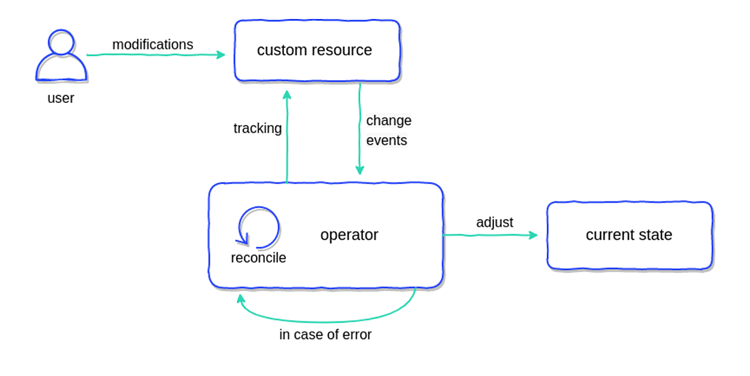
\includegraphics[width=160mm]{tech/operator-pattern.png}
    \caption{\emph{Operator Pattern model of Custom Controller and Resources interaction}}
    \label{op-pat}
\end{figure}

Whatever the use case, they serve the purpose of automating tasks beyond what Kubernetes provides out of the box. A model of the Operator pattern taken from the Container Solutions blog can be seen in Figure \ref{op-pat} \cite{op-pat-blog}. In order for Operators to carry out their intended functions, they need to be granted the necessary permissions.



\subsubsection{Role-Based Access Control}

Kubernetes environments use a Role-Based Access Control (RBAC) method to allow applications to perform certain tasks. Since the API Server acts as a mediator for all Kubernetes actions, the rules which describe a user's permissions use the verbs common to APIs like \emph{GET}, \emph{POST}, and \emph{DELETE} \cite{rbac}. First, applications (Controllers, Pods, Operators, etc) are assigned a Service Account. Roles can then be created which describe what actions any application assigned with that Role can take. Finally, Bindings can be created to link these Roles to specific Service Accounts. This method of permission granting will prove useful for the implementation of the Stretch Goal discussed in Section \ref{aims-and-obj}. These resources are discussed as part of a prototype Section \ref{rbac-prototype}.



\subsection{Languages}
There will be two main languages used in the creation of Heimdall, Go and YAML. They are the most commonly used languages when developing Kubernetes applications. This means that supporting documentation is plentiful, and experience with these languages is invaluable.  

\subsubsection{Go}

The Go Programming Language is an open-source language created by Google. It is predominately used to develop cloud and network services, command-line interfaces, web applications, and Developer Operations style projects \cite{go-dev}. Kubernetes Controllers fall under the latter category and since I already have an elementary proficiency with Go, this is the chosen language for Heimdall. The completion of this project will aid in increasing my knowledge and experience with Go, which will be beneficial for my future career.

\subsubsection{YAML}

YAML is a language highly similar to JSON. It is used frequently for defining configurations and is syntactically easy to use \cite{yaml-blog}. Similarly to Go, I have encountered and written YAML at Red Hat, and will be looking to further develop my skills with it during the creation of Heimdall. YAML is the language which defines the desired and actual state of Resources in Kubernetes as discussed in Section \ref{resources}. 

\subsection{Libraries}

Various libraries will be used for the development of Heimdall. Many of these are packaged up in the Software Development Kit discussed in Section \ref{osdk} so don't require discussion here. 


\subsubsection{Slack Go Client}

The Slack Client for Go (slack-go) allows interaction with Slack channels via code. This client will allow Heimdall to make a connection to a Slack Channel, and send custom notifications containing key information about the problem occurring. This client will be used in the Slack Prototype discussed in Section \ref{slack-watch-prototype}.

\subsubsection{Unstructured Package}

The Unstructured Package allows a Controller to watch and interact with any Kind of Resource. This is necessary for Heimdall as it needs to complete its tasks on any Resource in a cluster, regardless of Kind. This is achieved by setting a Watch on Resources with a specific label, such as \emph{heimdall: watching}. However, if a Controller is only set to watch a specific Kind, like \emph{Pod}, it will not be able to perform actions on Resources with that label if they do not also have the Kind \emph{Pod}. The Unstructured Package allows Heimdall to overcome this limitation and watch any Resource with the desired label.

\section{Tools}

The following section will provide an overview of the various tools used in the development of Heimdall, including online LaTeX editors and command line tools for interacting with Kubernetes clusters. It will also briefly describe the purpose and use of each tool and provide relevant background information.

\subsection{Overleaf}

Overleaf is an online LaTeX editor and is the tool used to create this report. It will also be the tool used to create the Semester Two report. LaTeX allows the creation of professionally formatted documents using plain text instead of formatted text as typically done with other document writing tools like Google Docs and Microsoft Word \cite{overleaf}.


\subsection{Operator SDK} \label{osdk}

Operator SDK is a Software Development Kit created for building Kubernetes Operators. It provides the necessary tools for the creation of custom Controllers and Resources (custom APIs) and generates a plethora of scaffolding code to get started on an Operator project \cite{osdk-overview}. During this scaffolding process, as seen in Figure \ref{osdk-img}, it can be specified whether or not to generate a Controller and Custom API. In the case of Heimdall, a Custom Resource is not needed so the flag to generate one is left to false.

\begin{figure}[H]
    \centering
    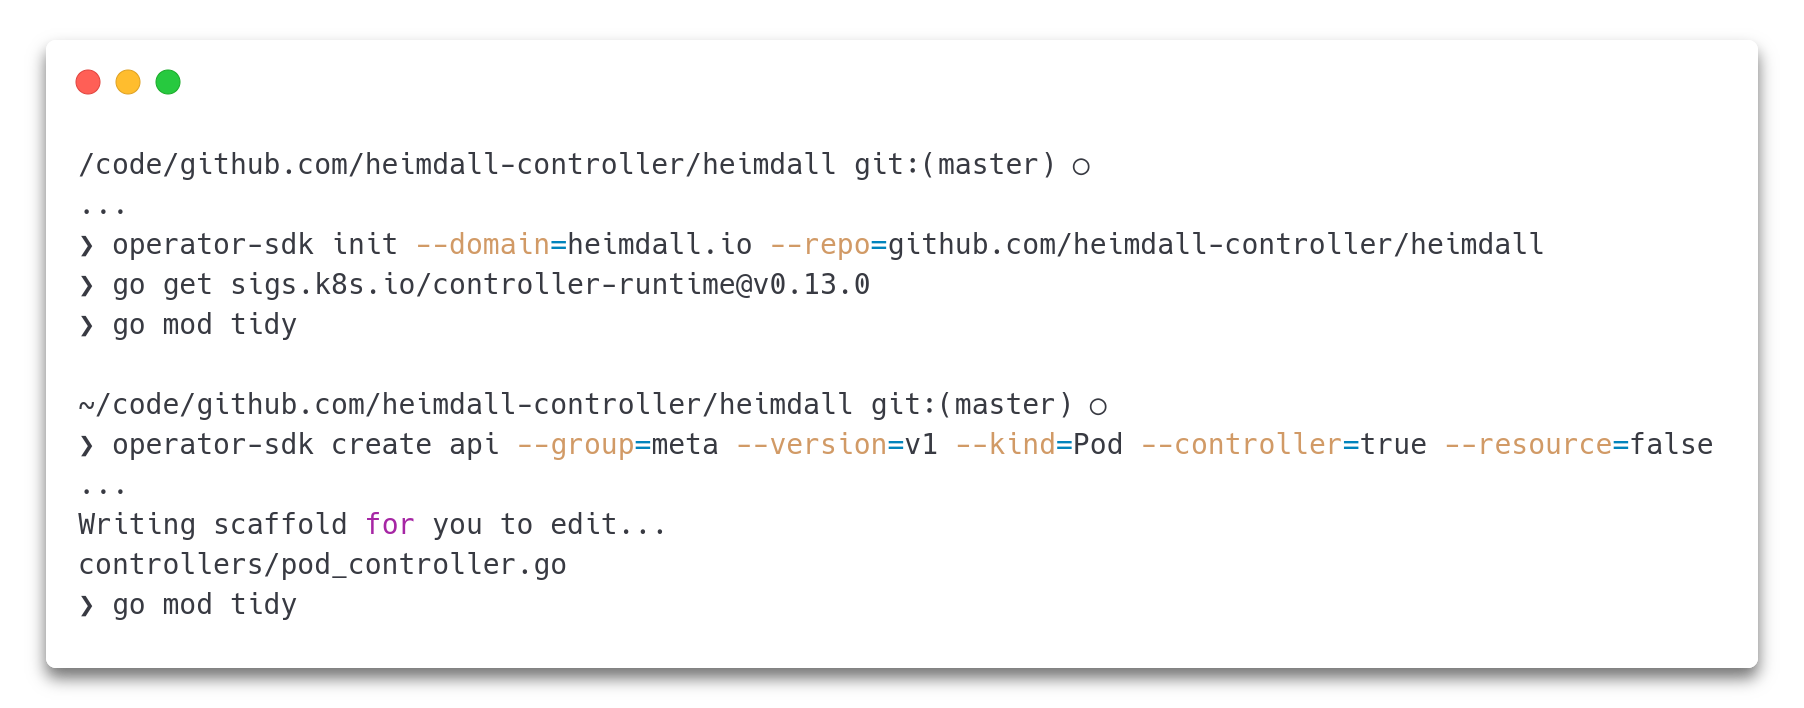
\includegraphics[width=160mm]{tools/osdk.png}
    \caption{\emph{Operator SDK Controller scaffolding via Command Line}}
    \label{osdk-img}
\end{figure}

Aside from code generation, Operator SDK also initialises the use of essential libraries like \emph{controller-runtime} and \emph{controller-tools}. These are sets of libraries that aid in the creation of custom Controllers and will be used extensively during the development of Heimdall.


\subsection{Minikube}

Minikube is a small open-source Kubernetes environment that uses one node (a virtual machine that Kubernetes runs on). It can be run locally and is typically used for the development of Kubernetes applications \cite{minikube-docs}. Minikube provides a dashboard which allows the use of a graphical user interface to configure the Kubernetes cluster and interact with resources. This will be the environment in which Heimdall will be tested. 

 
\subsection{Docker}

Docker is an open-source tool for deploying and shipping containerized applications that is commonly used in Kubernetes environments \cite{docker-overview}. For Heimdall, it will be used to build and push custom images for deployment to any Kubernetes environment. Docker will also be used in the release process of Heimdall as discussed in Section \ref{cicd}. Podman, another open-source tool created by Red Hat, can also be used for these purposes, but I have chosen to focus on improving my skills with Docker during Heimdall's development. Since the tools are largely very similar, skills with Docker are transferable to Podman.

\subsection{Kubectl}

Kubectl is a powerful command line tool used to interact with and manage Kubernetes clusters \cite{k8s-tools}. In the context of Heimdall, it will be used to deploy and manage the controller and other components in the cluster. It can also be used to troubleshoot and debug issues that may arise during development and deployment.


\subsection{Git and GitHub}

Git and GitHub are integral tools to implement a viable version control system as discussed in Section \ref{version-ctrl}. Git is the command line tool used to track changes to a code base while GitHub is the cloud-based platform that hosts repositories (projects) for tracking those changes. Git and GitHub are being utilized to implement the version control system for the Heimdall Controller, the report, and the prototypes. All of these repositories are stored in a GitHub Organization as discussed in Section \ref{open-source} in order to separate them from personal projects. Git and GitHub will be used to work on multiple different Heimdall features at once, track changes so they can be reverted if a bug is introduced, and host the Continuous Integration and Continuous Delivery systems via GitHub Actions as discussed in Sections \ref{cicd} and \ref{gha}


\subsection{GitHub Actions} \label{gha}

GitHub Actions provides a Continuous Integration and Continuous Delivery system for the automation of building, testing, and deploying software products. GitHub Action Workflows can be triggered upon a particular event like a push to the \emph{master} branch. Once triggered, it can perform actions like ensuring the project builds correctly, checking code formatting standards are met, and running tests. They can also be used to automate product releases \cite{github-actions}. This tool is already being utilized to build the LaTeX document on every Pull Request event and Push event for the Heimdall Report repository as seen in Appendix \hyperlink{appendix-e}{E}. This implementation provides a familiarity with GitHub Actions in preparation for Semester Two, while also ensuring the report is building successfully whenever changes are made.


\subsection{Jira}

Jira is a tool used by teams who follow the Agile methodology, as discussed in Section \ref{agile}. It provides templates for Scrum and Kanban boards for project management and is used to track pieces of work for this project. It offers features such as Sprint management, release creation, and automatic linking of GitHub Pull Requests to Jira Tasks. It was chosen over Trello due to these additional features, such as the ability to generate Burndown charts, which are not available in Trello without paid extensions.

\section{Proof of Concept}

Three prototypes were created to demonstrate the feasibility and functionality of the different components of Heimdall. This section will provide a brief discussion of each prototype's capabilities. While the creation process will not be detailed here, this information can be seen in each respective repository as seen in the GitHub Organization in Appendix \hyperlink{appendix-a}{A} and a supporting video demonstration can be viewed in Appendix \hyperlink{appendix-d}{D}.

\subsection{Slack and Watcher Prototypes} \label{slack-watch-prototype}

The Slack prototype is designed to send notifications to a Slack channel based on events occurring within a Kubernetes cluster, specifically Pod events. This demonstrates the possibility of out-of-cluster reactions to in-cluster events. The watcher prototype, on the other hand, demonstrates how a controller can watch specific resources such as Pods within a cluster and perform an action based on a specific event occurring to that resource. By merging these two prototypes together, it is possible to better demonstrate the potential capabilities of Heimdall and make the demonstration more effective. The combined functionality allows for external responses to be triggered by specific events occurring within the cluster, providing greater control and visibility into cluster activity.

\begin{figure}[H]
    \hypertarget{slack-notif}
    \centering
    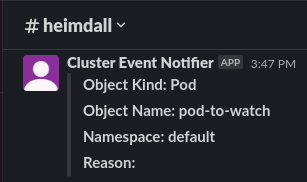
\includegraphics[width=85mm]{prototypes/slacknotif.png}
    \caption{\emph{Example Notification from Slack Prototype}}
    \label{slack-notif}
\end{figure}

Figure \ref{slack-notif} shows an example notification being sent to a Slack channel called \emph{\#heimdall}. This Pod is identified by a specific label, such as \emph{heimdall: watching}, and is watched by the Controller. When an event occurs on that Pod, the Controller extracts the Slack API Key from a Kubernetes secret stored in-cluster and sends a Slack notification to the configured Slack channel.


\subsection{RBAC Prototype} \label{rbac-prototype}

The RBAC Prototype demonstrates how to create and configure RBAC resources within a cluster through Controller code. As part of this prototype, an example operator called the \emph{changer-operator} was set up to continuously change the label of a Pod. The RBAC Prototype itself serves the function of creating Roles and Role bindings to reconfigure the permissions that the changer-operator possesses. The Controller logs of the creation of these Resources can be seen in Figure \ref{rbac-output}.

\begin{figure}[H]
    \hypertarget{rbac-output}
    \centering
    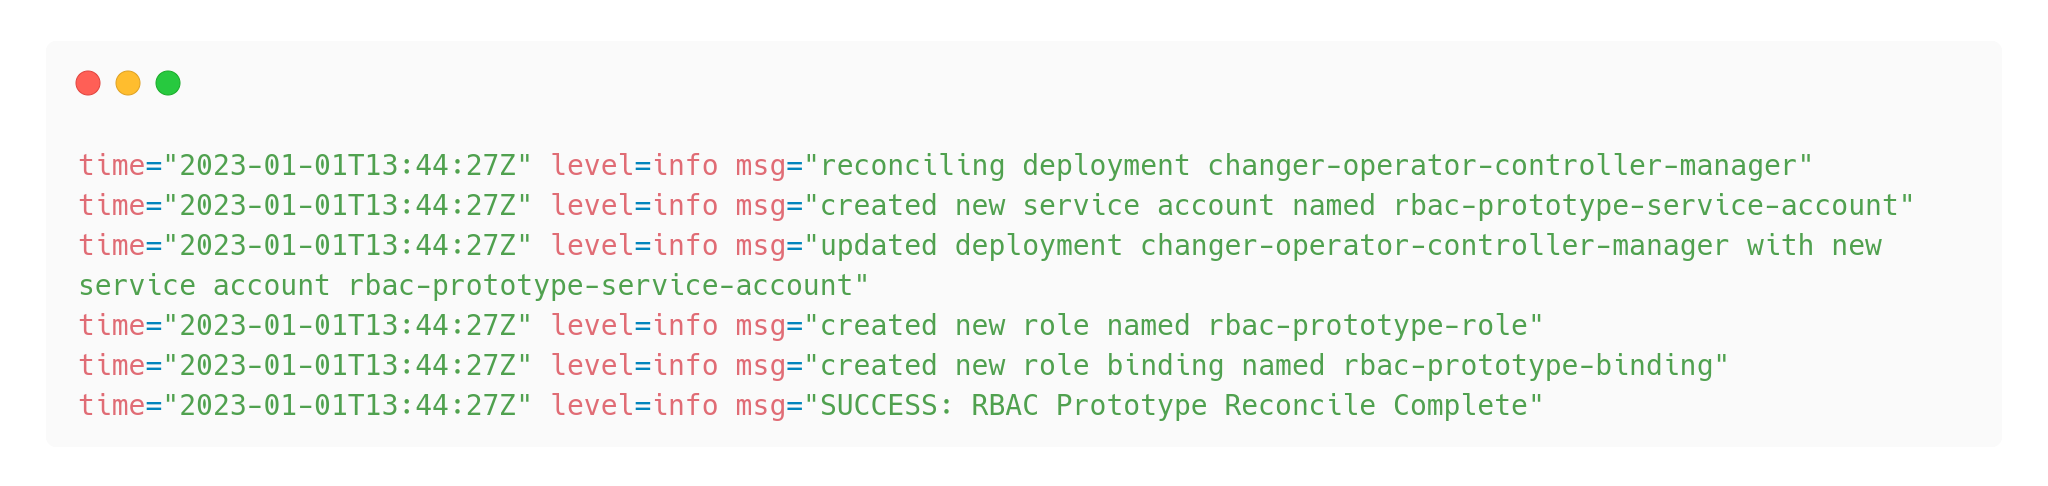
\includegraphics[width=165mm]{prototypes/rbac-output.png}
    \caption{\emph{RBAC Prototype Controller Output}}
    \label{rbac-output}
\end{figure}

This prototype serves to demonstrate that the permissions of an operator can be altered from a completely unrelated controller. This proves that Heimdall should, in some form, be able to alter an operator's RBAC configuration so that it is allowed or not allowed to make changes to a specific resource. While there will be many other factors in play during Heimdall's full implementation, this prototype serves as proof of feasibility that re-configuring the RBAC resources could be a possible method for accomplishing this task.

\section{Conclusion}
Overall, it has been a fantastic opportunity to learn about the process of developing a product in an Agile environment, and I'm excited to have the chance to contribute a real open-source solution to a problem commonly experienced in the industry. Working with mentors from Red Hat and my supervisor was a huge help throughout the semester, and I'm grateful for the guidance and support they provided. Looking ahead to next semester, I'm eager to get straight into the development of Heimdall and tackle the various challenges that lie ahead. My plan is to start by integrating a better version of the Slack prototype, and then focus on integrating the unstructured package so that it can be used with any resource kind. From there, I will turn my attention to dynamically re-configuring operator permissions and identifying the source of events on a resource. \\\par The process of learning how to manage a product's development was both challenging and rewarding. Working in an Agile way was an interesting experience, and it was gratifying to see how my understanding and use of Agile principles improved over the course of the semester. The creation of prototypes was especially challenging, as it required me to think creatively and carefully consider the needs of the final solution. However, this process was also productive, as it helped me to better understand the requirements and constraints of Heimdall and to identify the best approach for addressing the problem. With this knowledge and experience, I am excited to continue the development of Heimdall and bring it to fruition as a valuable open-source solution for the industry.


\bibliographystyle{alpha}


\clearpage
\begin{thebibliography}{9}


\bibitem[What is Agile?, 2022]{what-is-agile}
\emph{Atlassian}, \\Available at: https://www.atlassian.com/agile 

\bibitem[Operator Pattern, 2022]{operator-pattern}
\emph{Kubernetes}, \\Available at: https://kubernetes.io/docs/concepts/extend-kubernetes/operator/

\bibitem[IBM API-Connect, 2022]{understanding-apis}
\emph{Understanding rate limits for APIs and Plans}, \\Available at: https://www.ibm.com/docs/en/api-connect/10.0.1.x?topic=connect-understanding-rate-limits-apis-plans

\bibitem[I. Sommerville, 2021]{agile-book}
\emph{Engineering Software Products: An Introduction to Modern Software Engineering}, 2021.
  
\bibitem[Kubernetes Overview, 2022]{k8s-overview}
\emph{Kubernetes}, \\Available at: https://kubernetes.io/docs/concepts/overview/  

\bibitem[Red Hat Developer, 2020]{rhoam-overview}
\emph{Red Hat OpenShift API Management}, Red Hat, 2020. \\Available at: https://developers.redhat.com/products/red-hat-openshift-api-management/overview

\bibitem[K8s Objects, 2022]{k8s-obj}
\emph{Understanding Kubernetes Objects}, Kubernetes. \\Available at: https://kubernetes.io/docs/concepts/overview/working-with-objects/kubernetes-objects/
  
\bibitem[Y. Maharjan, 2020]{k8s-rolling}
\emph{How Rolling and Rollback Deployments work in Kubernetes}, Medium, 2020. \\Available at: https://yankeexe.medium.com/how-rolling-and-rollback-deployments-work-in-kubernetes-8db4c4dce599 

\bibitem[Custom Resources, 2022]{cust-res}
\emph{API Extension}, Kubernetes. \\Available at: https://kubernetes.io/docs/concepts/extend-kubernetes/api-extension/custom-resources/ 
  
\bibitem[Controllers, 2022]{ctrlrs-ref}
\emph{Kubernetes Architecture}, Kubernetes. \\Available at: https://kubernetes.io/docs/concepts/architecture/controller/ 
  
\bibitem[Using RBAC Authorization, 2022]{rbac}
\emph{API Access Control}, Kubernetes. \\ Available at: https://kubernetes.io/docs/reference/access-authn-authz/rbac/  

\bibitem[P. Perzyna, 2020]{op-pat-blog}
\emph{Kubernetes Operators Explained}, \\Available at: https://blog.container-solutions.com/kubernetes-operators-explained
  
\bibitem[Go Docs, 2022]{go-dev}
\emph{The Go Programming Language}, \\Available at: https://go.dev/

\bibitem[Understanding Automation, 2021]{yaml-blog}
\emph{What is YAML?}, Red Hat. \\Available at: https://www.redhat.com/en/topics/automation/what-is-yaml

\bibitem[Overleaf About Us, 2022]{overleaf}
\emph{About us}, Overleaf, Online LaTeX Editor. \\Available at: https://www.overleaf.com/about 

\bibitem[Operator SDK Overview, 2022]{osdk-overview}
\emph{Operator SDK Documentation},\\ Available at: https://sdk.operatorframework.io/docs/overview/

\bibitem[Minikube Docs, 2022]{minikube-docs}
\emph{Minikube}, \\Available at: https://minikube.sigs.k8s.io/docs/

\bibitem[Docker Overview, 2022]{docker-overview}
\emph{Docker Documentation}, 2022. \\Available at: https://docs.docker.com/get-started/overview/
  
\bibitem[Kubernetes Tools]{k8s-tools}
\emph{Install Tools}, Kubernetes. \\Available at: https://kubernetes.io/docs/tasks/tools/kubectl

\bibitem[Learn GitHub Actions, 2022]{github-actions}
\emph{Understanding GitHub Actions}, GitHub Docs. \\Available at: https://docs.github.com/en/actions/learn-github-actions/understanding-github-actions

\bibitem[P. Gorbachenko, 2021]{func-vs-nonfunc}
\emph{Functional vs Non-Functional Requirements}, Enkonix. \\Available at: https://enkonix.com/blog/functional-requirements-vs-non-functional/

\bibitem[Agile Alliance, 2015]{user-stories}
\emph{Agile Alliance}, Dec. 17, 2015. \\Available at: https://www.agilealliance.org/glossary/user-stories/
  
\bibitem[Scrum Guides, 2021]{scrum-guides}
\emph{Scrum Guide}, Scrum Guides. \\Available at: https://scrumguides.org/scrum-guide.html
  
\bibitem[Red Hat, 2022]{ci-cd}
\emph{What is CI/CD?}, Red Hat. \\Available at: https://www.redhat.com/en/topics/devops/what-is-ci-cd

\end{thebibliography}

\clearpage
\section*{Appendices}
\subsubsection*{A Heimdall GitHub Organization} \label{appendix-a}
\hypertarget{appendix-a}{https://github.com/heimdall-controller}

\subsubsection*{B Slack Prototype GitHub Repository} 
\hypertarget{appendix-b}{https://github.com/heimdall-controller/slack-prototype}

\subsubsection*{C RBAC Prototype GitHub Repository} 
\hypertarget{appendix-c}{https://github.com/heimdall-controller/rbac-prototype}

\subsubsection*{D Prototype YouTube Demonstration} \label{appendix-d}
\hypertarget{appendix-d}{https://www.youtube.com/watch?v=m8tXulOU8y4}

\subsubsection*{E Heimdall Report GitHub Repository} \label{appendix-e}
\hypertarget{appendix-e}{https://github.com/heimdall-controller/heimdall-report}

\subsubsection*{F Sprint Review Document} \label{appendix-f}
\hypertarget{appendix-f}{https://docs.google.com/document/d/1-2GoGv4KZo0Blm5s8Z0NAZyT0wclrPDSab4et4ho7jg/edit?usp=sharing}



\end{document}